% ****** Start of file aipsamp.tex ******
%
%   This file is part of the AIP files in the AIP distribution for REVTeX 4.
%   Version 4.1 of REVTeX, October 2009
%
%   Copyright (c) 2009 American Institute of Physics.
%
%   See the AIP README file for restrictions and more information.
%
% TeX'ing this file requires that you have AMS-LaTeX 2.0 installed
% as well as the rest of the prerequisites for REVTeX 4.1
%
% It also requires running BibTeX. The commands are as follows:
%
%  1)  latex  aipsamp
%  2)  bibtex aipsamp
%  3)  latex  aipsamp
%  4)  latex  aipsamp
%
% Use this file as a source of example code for your aip document.
% Use the file aiptemplate.tex as a template for your document.
\documentclass[%
 aps,
 %jmp,%
 %prb,
 prl,
 amsmath,amssymb,
 %preprint,%
 %superscriptaddress,
 reprint,%
 %floatfix,
%author-year,%
%author-numerical,%
]{revtex4-1}
%]{article}

\usepackage{graphicx}% Include figure files
\usepackage{dcolumn}% Align table columns on decimal point
\usepackage{bm}% bold math
%\usepackage[mathlines]{lineno}% Enable numbering of text and display math
%\linenumbers\relax % Commence numbering lines

% Alter some LaTeX defaults for better treatment of figures:
    % See p.105 of "TeX Unbound" for suggested values.
    % See pp. 199-200 of Lamport's "LaTeX" book for details.
    %   General parameters, for ALL pages:
    \renewcommand{\topfraction}{0.9}    % max fraction of floats at top
    \renewcommand{\bottomfraction}{0.8}    % max fraction of floats at bottom
    %   Parameters for TEXT pages (not float pages):
    \setcounter{topnumber}{2}
    \setcounter{bottomnumber}{2}
    \setcounter{totalnumber}{4}     % 2 may work better
    \setcounter{dbltopnumber}{2}    % for 2-column pages
    \renewcommand{\dbltopfraction}{0.9}    % fit big float above 2-col. text
    \renewcommand{\textfraction}{0.07}    % allow minimal text w. figs
    %   Parameters for FLOAT pages (not text pages):
    \renewcommand{\floatpagefraction}{0.7}    % require fuller float pages
    % N.B.: floatpagefraction MUST be less than topfraction !!
    \renewcommand{\dblfloatpagefraction}{0.7}    % require fuller float pages
    % remember to use [htp] or [htpb] for placement
    \setlength{\abovecaptionskip}{0pt}
    \setlength{\belowcaptionskip}{0pt}
    \setlength{\parskip}{0pt}
    \setlength{\textfloatsep}{1pt} 

\begin{document}
%\title{Reduction of turbulent fluctuations and crossphase through driven sheared flow on the Large Plasma Device}
\title{Observation of improved and degraded confinement with driven flow on the LAPD}
\author{D.A. Schaffner}
\affiliation{Department of Physics and Astronomy, University of California, Los Angeles.}
\author{T.A Carter}
\affiliation{Department of Physics and Astronomy, University of California, Los Angeles.}
\author{D.S. Guice}
\affiliation{Department of Physics and Astronomy, University of California, Los Angeles.}
\author{J. Maggs}
\affiliation{Department of Physics and Astronomy, University of California, Los Angeles.}
\author{S. Vincena}
\affiliation{Department of Physics and Astronomy, University of California, Los Angeles.}
\author{B. Friedman}
\affiliation{Department of Physics and Astronomy, University of California, Los Angeles.}
\author{G.D. Rossi}
\affiliation{Department of Physics, University of Texas, Austin}

\date{\today}% It is always \today, today,
             %  but any date may be explicitly specified

\begin{abstract}
Continuous control over azimuthal flow and shear in the edge of the Large Plasma Device (LAPD) has been acheived using a biasable limiter allowing a detailed study of the effect of flow shear on turbulence and transport in LAPD, extending previous work~\cite{carter09}. LAPD rotates spontaneously in the ion diamagnetic direction (IDD); positive limiter bias first reduces, then minimizes (producing a near-zero shear state), and finally reverses flow into the electron diamagnetic direction (EDD). Confinement---decreases in radial cross-field transport---are shown to vary continuously with shearing rate. Comfinement degredation is observed in the minimum shearing state and confinment improvement in higher shearing states for both flow directions. Such improvement is shown to begin at shearing rates less than the no-shear turbulent autocorrelation rate. This suppression is dominated by decreases in low-frequency $>10$kHz density fluctuations and a reduction in the radial extent of correlation structures. An increase in fluctuations for the highest shearing states is observed with the emergence of a 10kHz coherent mode; however, overall flux is unchanged as isat/E-field crossphase nulls out radial transport. The variations of density fluctuation and radial correlation length are fit to power-law functions for comparison to simple shearing effects models.
\end{abstract}

\maketitle
%\section{Introduction}  No need for section titles in PRL, save space

%% Need to start with discussion of H-mode, role of flow.  Cite BDT, recent reviews of flow-shear interaction (Terry, Diamond, Tynan).  Move immediately to set up why this study is unique

The effect of flow and flow shear on plasma turbulence has long been studied as a mechanism for turbulence reduction and increased particle confinement in both tokamaks and linear machines.  The most dramatic observed effect of cross-field flow is the creation of a higher confinement state, called an H-mode, first observed on ASDEX\cite{wagner82} and later on other tokamaks such as the Continuous Current Tokamak (CCT)\cite{taylor89,tynan92} and DII-D\cite{groebner90,moyer95}. While some plasma machines rely on a spontaneous flow for study\cite{tynan06}, other machines including TEXTOR\cite{boedo00} and LAPD\cite{maggs07,carter09} have developed external biasing mechanisms to produce radial electric fields which can drive controllable azimuthal flow by $E \times B$ drift\cite{weynants93}.

Theoretical investigation into the nature of effect of sheared flow has focused mainly on its influence on turbulent fluctuations \cite{biglari90} and on the crossphase between electric field and an advected quantity, such as density in the case of particle flux \cite{ware96,terry01}. Fluctuation suppression by shear is thought arise through the reduction in radial correlation length(i.e., shearing of turbulent eddies) while relative phasing between fluctuation electric field and density can either promote overall inward or outward motion of particles, or zero out such change on average. The simplest mode non-specific models for the effect of shearing on turbulent fluctuations predict a power law decrease\cite{biglari90}, while crossphase can have an even stronger scaling\cite{terry01}.

Biasing experiments have been previously conducted on LAPD. In one, an inward pointing electric field produced by chamber biasing demonstrated that increased flow shear resulted in turbulent modification and increased particle confinement\cite{carter09}. However, penetration of the electric field was low until high biases resulting in a sudden transition from initial states to confined states so continous control of flow was never achieved. In another, it was shown that a small biased annulus could produce sheared flows within the main column of the plasma\cite{zhou12}. A new biasing mechanism combines these approaches allowing for a continuous transition from a low shear edge state in the IDD---LAPD's natural state---to a zero shear state, to a high shear state in the EDD. With this smooth control of flow shear, we can carefully observe the effect of shear on turbulent fluctuations, particle flux, and gradient length scale to a level of detail not yet previously achieved.

In this letter, we report on the observation of improved and degraded cross-field confinement as a function of sheared flow, $\omega_{s}$, ranging from zero to five times a no-shear turbulent autocorrelation rate, $\Delta \omega_{d}$. This confinement occurs regardless of flow direction and is demonstrated through both gradient scale length variation of density profiles and by tubulent particle flux measurements. We show that radial correlation length, particle flux, and density fluctuation power all decrease with $\omega_{s}$ and decreases begin for $\omega_{s} < \Delta \omega_{s}$. The overall decrease in radial flux here is dominated by decreases in density fluctuations and reduction of the radial correlation length of turbulent structures for frequencies less than 10kHz. In this range, crossphase between density and azimuthal electric field fluctuations remain near zero for all shearing rates which tends to maximize outward radial turbulent transport. We do note the emergence of a coherent mode at high shear with frequencies above 10kHz that originates in the region of peak flow. Fluctuations from this mode appear to increase density fluctuations above 10kHz, but do not appear to contribute to flux as crossphase in this region is aligned to minimize any transport on average. We note that electric field fluctuations appear to be much less affected by shearing changes than density. Lastly, we show fits of density fluctuations and radial correlation length to a power-law decay for comparison to theory \cite{biglari90}.

The Large Plasma Device \cite{gek91} (LAPD) is a 20m by 1m cylindrical linear device with a 54cm wide barium-oxide coated nickel cathode pulsed at 1Hz to produce a 45eV electron beam which ionizes the helium gas in the chamber. A column long plasma of density about $5 \times 10^{12}$ cm$^{-3}$ and temperature of 5eV is produced. The field for this experiment was set to 1000G. To produce the bias, four quarter annulus aluminum plates are inserted half a meter axially beyond the cathode creating an iris-like boundary condition with an aperature of 26cm between the cathode-anode surface and the main plasma chamber. A pulse power circuit connected to a capacitor bank supplies a 5ms bias during the 15ms plasma discharge. Bias ranges from a floating potential of 35V to 230V referenced from the cathode. Measurements of ion saturated current (isat---proxy for density) and floating potential are taken with a 9-tip flush surface tantalum probe while temperature and plasma potential is taken by swept Langmuir probe.

Azimuthal flow and shear are controlled by adjusting the voltage on the limiter plates. When voltages on the limiter are less than the voltage of the anode---as is the case for LAPD's spontaneous flow state---an overall azimuthal flow occurs in the IDD as shown in Fig.~\ref{fig:velocity_flowshear} with velocities peaking just outside the limiter edge. When the voltage on the limiter is brought near anode potential, flow and flow shear zero out. Voltages above anode produce electron diamagnetic direction flows peaked at the limiter edge. The voltage on the power supply cannot be set below the floating potential as the plasma tends to charge the capacitor banks.

Measurements of isat and particle flux are taken for each bias flow state. Values are averaged over a range from 27 to 31cm, a region where such averaged flow and flow shear scale linearly with limiter bias and is outside the limiter edge to avoid any possible effects from primary electrons. An autocorrelation rate of $\Delta \omega_{t} = $ 28kHz is calculated from no-shear isat fluctuations by taking the half-width at half max of a Hilbert transform of the isat autocorrelation function.

Density gradient length scale is calculated by $L_{n} = \lvert \nabla \ln n \rvert ^{-1}$ from isat radial profiles while particle flux, $\Gamma_{p} = \langle \tilde{n} \tilde{v_{r}} \rangle = \langle \tilde{n} \tilde{E_{\theta}} \rangle /B$, can be calculated spectrally as\cite{powers74}, 
\begin{equation}
\Gamma_{p} = \frac{2}{B} \int^{\infty}_{0} \lvert n(\omega) \rvert \lvert E_{\theta}(\omega) \rvert \gamma_{n,E_{\theta}}(\omega) \cos [\phi_{n,E_{\theta}}(\omega)] d\omega
\label{eq:fluxint}
\end{equation}
which allows for separate analysis of fluctuations, crossphase and coherency.

The first clear result is a degredation of confinement from the spontaneous state followed by improved confinement as bias is increased, as indicated by $\langle L_{n}\rangle$ in Fig.~\ref{fig:densgrad}. Beginning at 9cm with no bias, $\langle L_{n}\rangle$ reaching a scale length peak of about 15cm at the bias corresponding to zero shear. As bias
\begin{figure}
\begin{center}
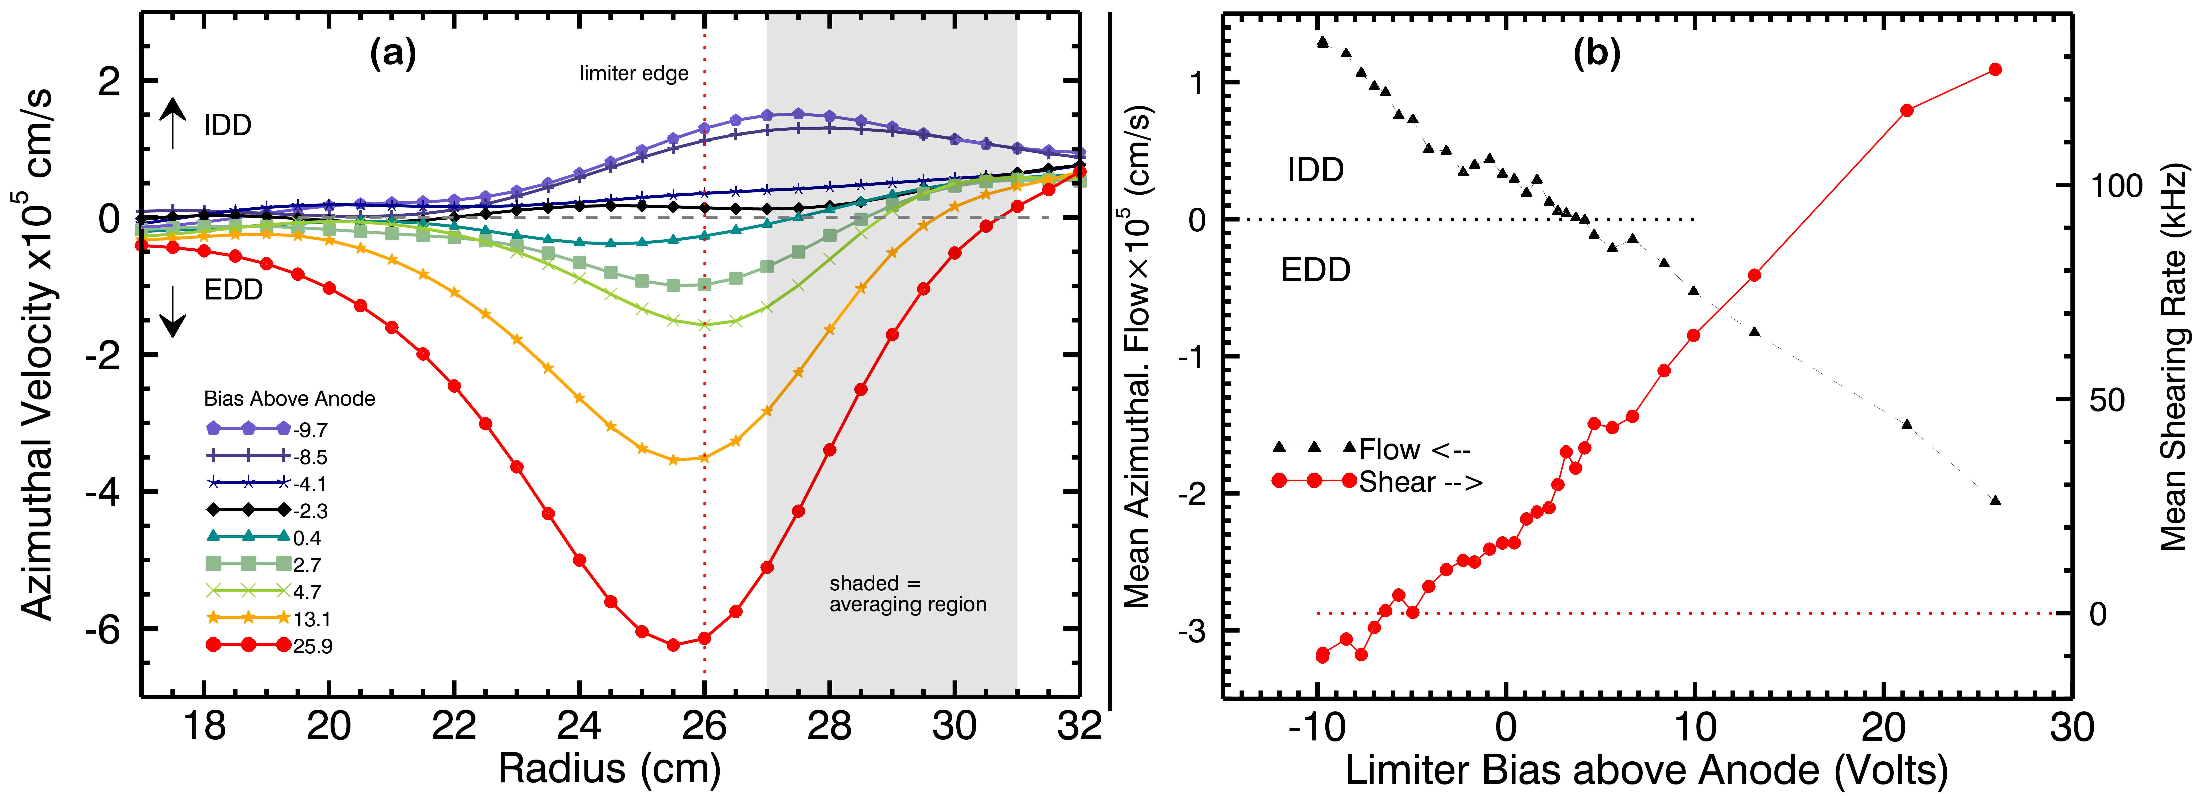
\includegraphics[width=8.5cm]{velocity_flowshear.pdf}% Here is how to import EPS art
\caption{\label{fig:velocity_flowshear} (a) Velocity profiles using plasma potential from swept measurements. (b) Nearly linear scaling of flow (black) and shearing (red) versus limiter bias.}
\end{center}
\end{figure}
increases, the density gradient gradually steepens saturating at about 5cm. The initial scale length value and saturated values are consistent with previous biasing experiments done on the LAPD\cite{carter09}, but rather than see a gradual change like here, a sharp threshold was observed. This gradual transition can be observed beause the new design allows for continous variation of flow at the plasma edge. In the previous experiment, a threshold was observed not because of an inherent dependence on a shear value, but because of lack of penetration of cross-field current---and thus flow---from the chamber edge to the plasma source until a high enough bias was reached. By placing the limiters closer to the core plasma edge edge, we can establish cross-field currents at lower bias values than before.

\begin{figure}
\begin{center}
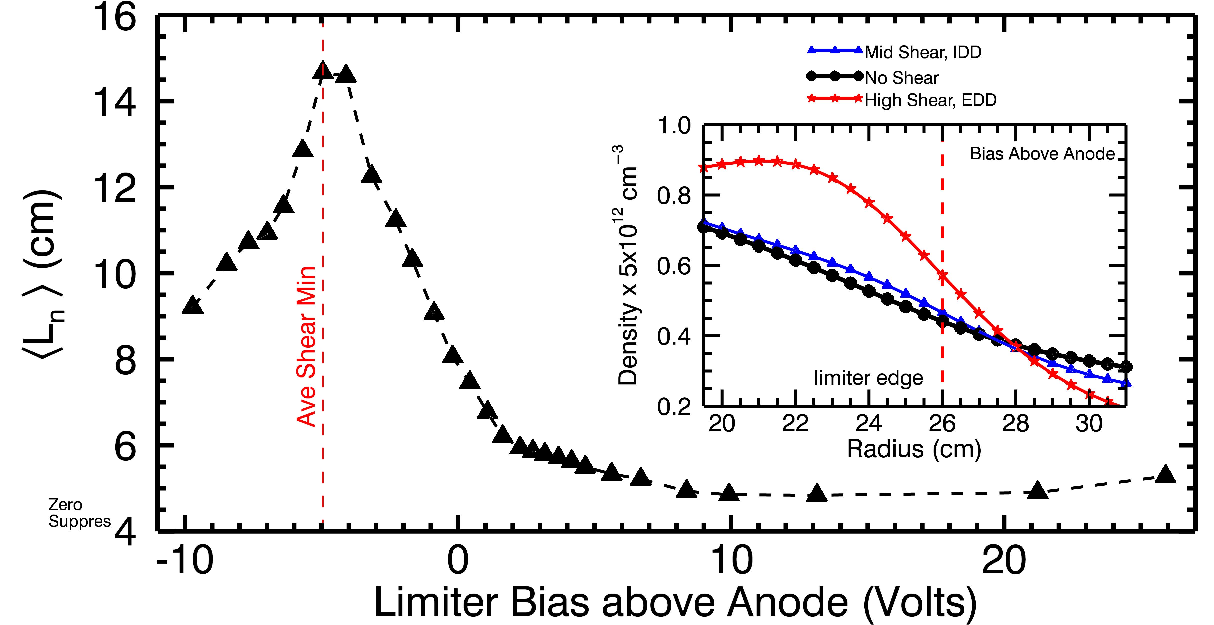
\includegraphics[width=8.5cm]{densgrad.pdf}% Here is how to import EPS art
\caption{\label{fig:densgrad} Density gradient length scale versus limiter bias. Inset shows density profile relaxing then steepening again with bias.}
\end{center}
\end{figure}

\begin{figure}
\begin{center}
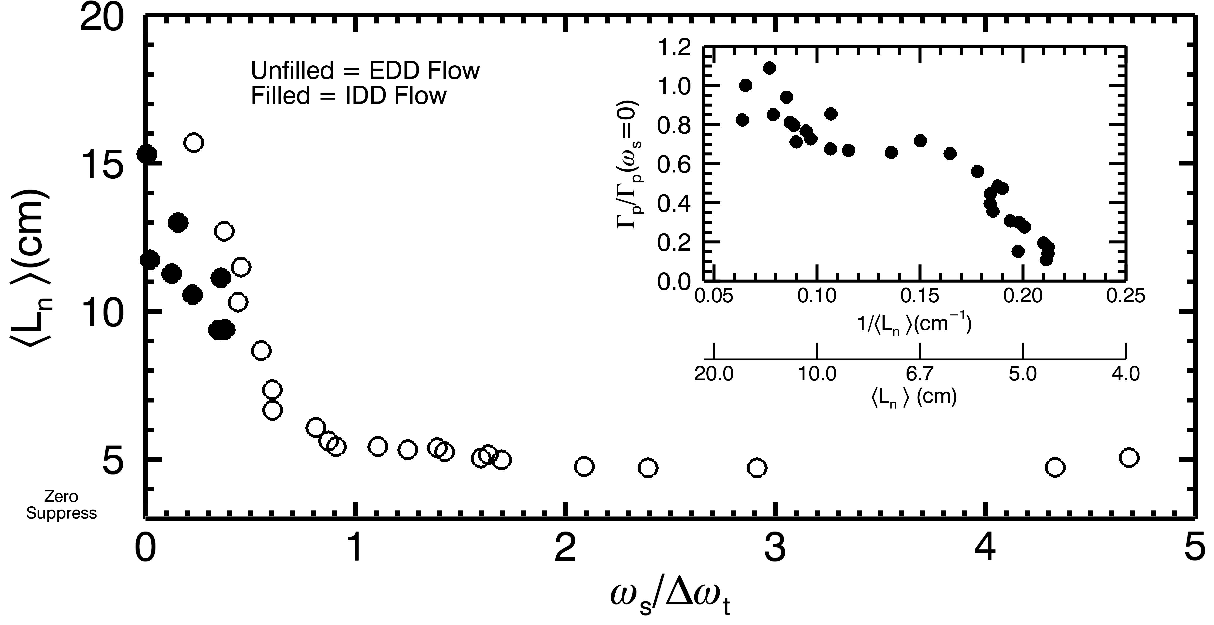
\includegraphics[width=8.5cm]{shearandgrad.pdf}% Here is how to import EPS art
\caption{\label{fig:shearandgrad} Gradient scale length versus shearing rate. Inset shows correlation of gradient scale length and turbulent particle flux. Note how this data is inconsistant with a Fick's Law like diffusion, which would be identified by a linearly increasing flux with gradient.}
\end{center}
\end{figure}

Given the linear relationship between limiter bias and average shear flow, we can compare $\langle L_{n} \rangle$ to shearing rate, $\omega_{s}$, normalized to $\Delta \omega_{d}$ as in Fig.~\ref{fig:shearandgrad}. Confinement improvement occurs continuously and gradually with $\omega_{s}$ and reaches a saturated state of 80\% initial levels for $\omega_{s} \approx \Delta \omega_{d}$. Improved confinement does not depend on flow direction as both IDD and EDD flow points lie on the same curve.

The change in confinement can be connected to a change in the fluctuation properties of the plasma which dictate the turbulent flux. Fluctuation power in isat can be seen in the spectrum of Fig.~\ref{fig:powercontour}
\begin{figure}
\begin{center}
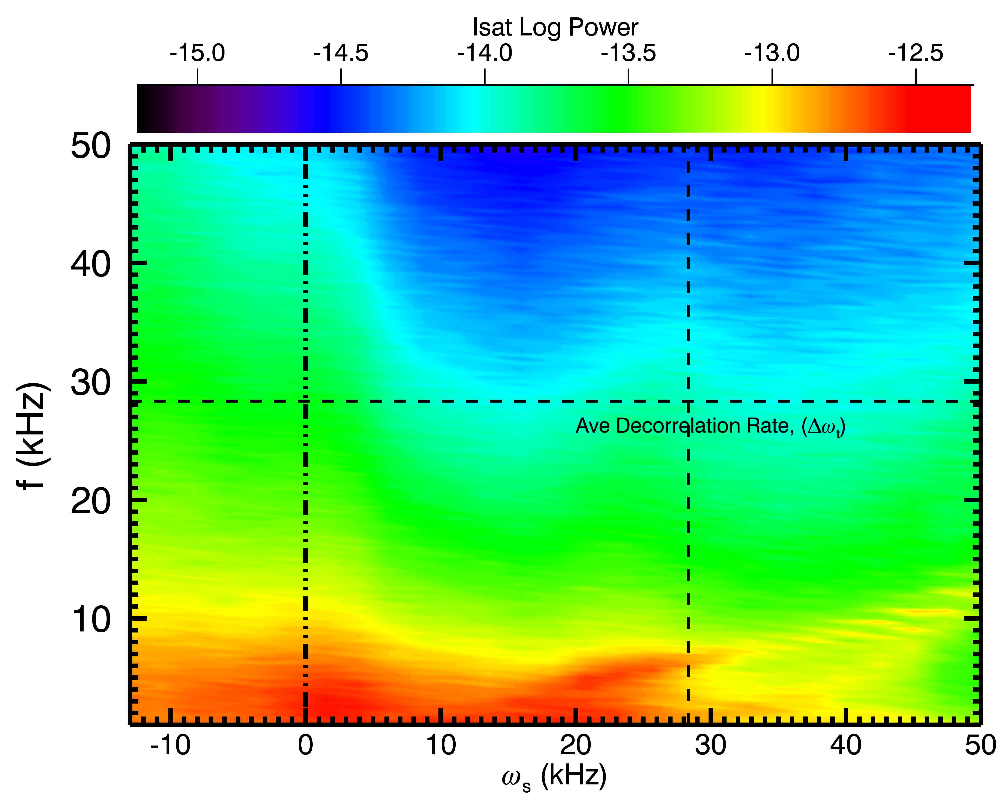
\includegraphics[width=8.5cm]{powercontour.pdf}% Here is how to import EPS art\
\caption{\label{fig:powercontour} Contour plot of log isat fluctuation power versus shearing rate and frequency. Dashed lines show location of decorrelation rate.}
\end{center}
\end{figure}
Most of the power is located in frequencies $<10$kHz and in this range, power decreases overall with increasing shearing rate. A decrease of about one order of magnitude is seen between the lowest shearing point and the high shear regime. Above 10kHz, power drops off considerably; however, just beyond $\omega_{s} = \Delta \omega_{s}$, a coherent mode emerges with a frequency that begins at about 10kHz and increases linearly with shearing. The power at these high shearing rates is almost entirely located within this mode.

The changes in $L_{n}$ and fluctuations are indicative of an overall change in particle flux. This flux can be directly measured by correlating isat with radial flow---$E \times B$ flow---using an $E_{\theta}$ derived from two floating potential tips on either side of the isat measuring tip and rewritten in terms of the integral in \eqref{eq:fluxint}. Like $L_{n}$, flux decreases with shearing rate as in Fig.~\ref{fig:fluxvsshear}; however, while flux decrease begin immediately with shearing, the decrease is not as fast as $L_{n}$ with saturation not occuring until at least $\omega_{s} > 2\Delta \omega_{d}$. Flux decreases do not depend on flow direction either as again both IDD and EDD points fit on the same curve.

\begin{figure}
\begin{center}
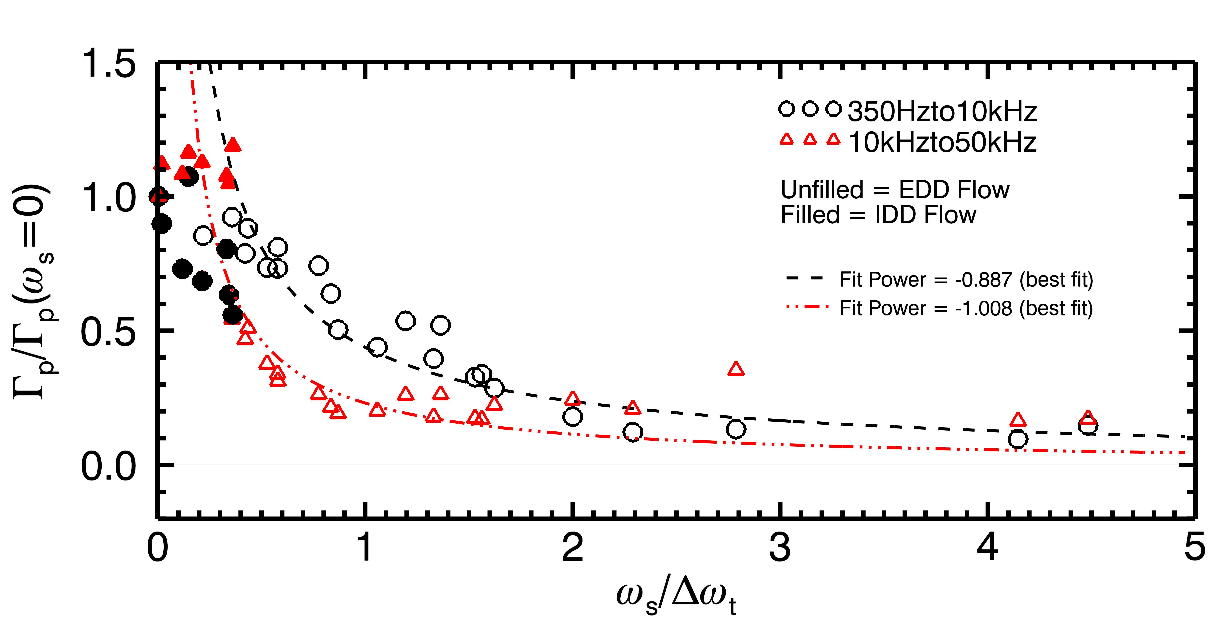
\includegraphics[width=8.5cm]{fluxvsshear.pdf}% Here is how to import EPS art
\caption{\label{fig:fluxvsshear} Particle flux normalized to no-shear flux as a function of normalized shearing rate. Filled symbols represent points with flow in IDD.}
\end{center}
\end{figure}

%When the flux is bandwidth limited, a difference emerges. The flux from 350Hz to 10kHz, where most of the fluctuation power is located, drops off gradually, %hitting its minimum only at a shearing rate about three times the decorrelation rate. Higher bandwidth though, 10kHz to 50kHz, drops off faster, nearing its %minimum when shearing equals decorrelation rate. Best fit lines from log-log plots of these scatters using a power law form of $\left(\omega_{s}/\Delta %\omega_{t}\right)^{\alpha}$ yield exponents of $\alpha = -0.887$ for the low bandwidth flux and about $\alpha = -1.008$ for the high bandwidth flux. 

\begin{figure}
\begin{center}
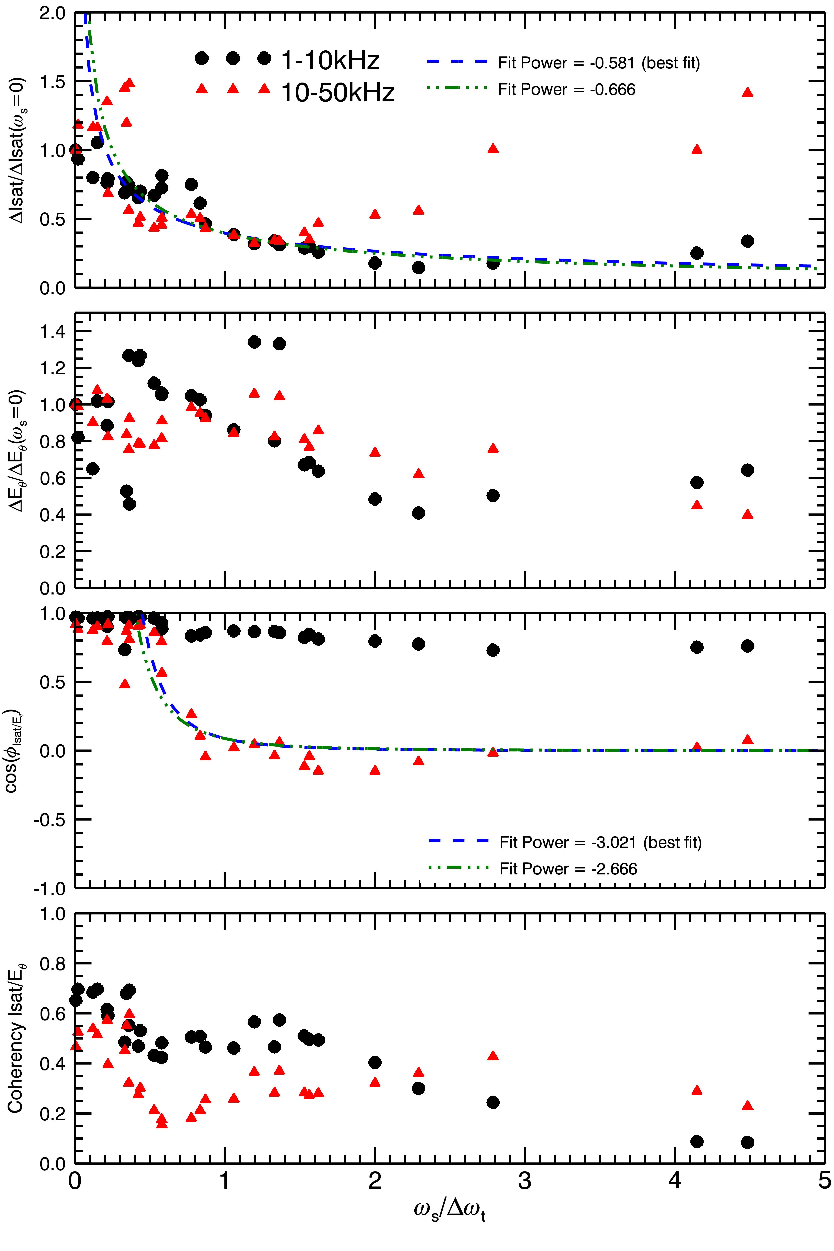
\includegraphics[width=8.5cm]{fluxcomps.pdf}% Here is how to import EPS art
\caption{\label{fig:fluxcomps} Components of particle flux versus shearing rate including isat/Density fluctuation power(a), electric field fluctuation power(b), crossphase(c) and coherency(d) with black points for low frequency, red for high.}
\end{center}
\end{figure}

\begin{figure}
\begin{center}
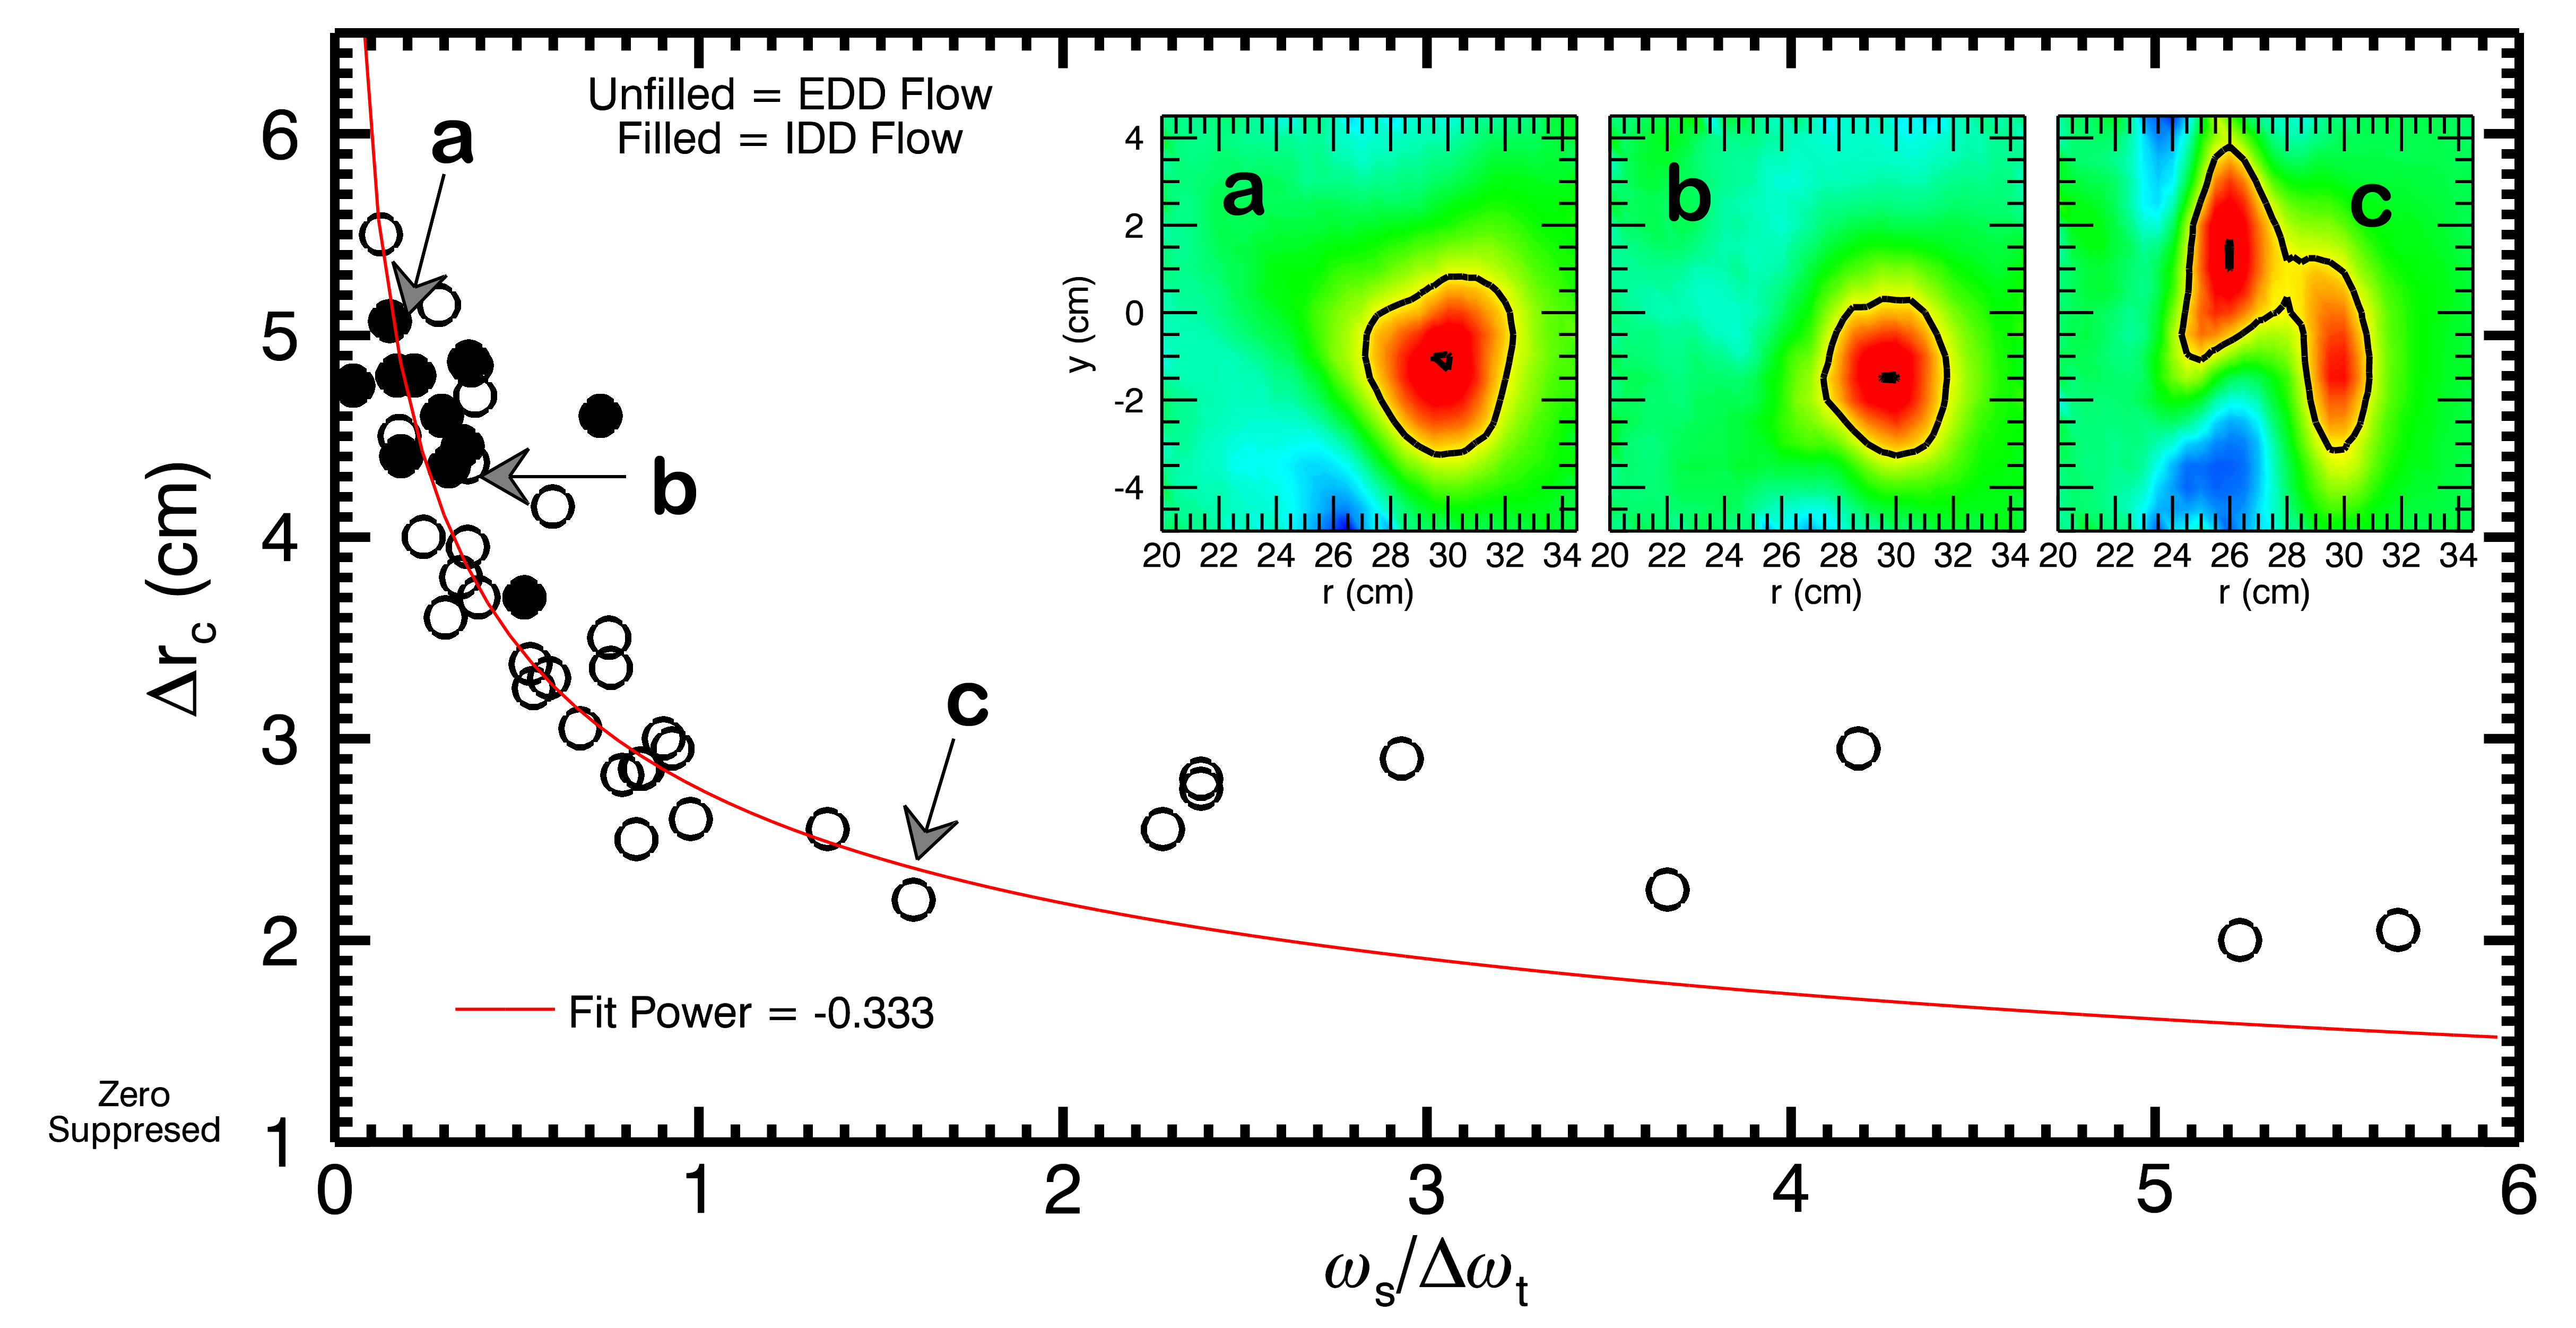
\includegraphics[width=8.5cm]{radcorr.pdf}% Here is how to import EPS art
\caption{\label{fig:radcorr} Radially correlation lengths with reference probes at 28,29,30,31 or 32cm. Inset shows 2D correlation structure for IDD flow, no shear and high EDD flow. A mode pattern is seen at flow peak (26cm).}
\end{center}
\end{figure}

The calculated flux can be analyzed by its fluctuation and phase components separately as in Fig.~\ref{fig:fluxcomps}. The top two plots show fluctuation power---isat and azimuthal electric field ($E_{\theta}$)---as functions of normalized shearing rate, while the bottom two show crossphase and coherency between the two fluctuating quantities. As expected from the power contour plot, isat fluctuations decrease with shearing for frequencies $<10$kHz. Concurrently, $\cos(\phi_{isat,E_{\theta}})$ for this bandwidth remains steady at nearly 1.0. Thus, since fluctaution power is concentrated in the low frequencies, overall flux is predominately suppressed by decreases in isat fluctuations, not crossphase. Note, however, isat fluctuations appear to increase beyond a normalized shearing of 2.0. These increases, however, are almost entirely from $>10$kHz contributions suggesting that they originate from the coherent mode. Comparing to Fig.~\ref{fig:fluxvsshear}, it is clear these flucutations do not contribute significantly to the flux. For high frequencies $\cos(\phi_{isat,E_{\theta}})$ is nearly zero for $\omega_{s} > \Delta \omega_{d}$. Thus, despite increased fluctuations at high shear, no overall flux is observed. 

%For low bandwidth, isat power decreases gradually, with a power fit of $\alpha = 0.581$. Crossphase, on the other hand, does not decrease. In this bandwidth %then, decreases in flux are primarily due to decreasing turbulent power. For high bandwidth flux, though, the opposite appears to be true. While isat %fluctuations do decrease initially, they actually begin to increase at high shearing rates. In this case, flux suppression is primarily due to the drop in %crossphase and to some extent coherency, regardless of growing turbulent power. A fit to this high frequency crossphase calculation yields $\alpha = -3.021$.  %Electric field fluctuations, meanwhile, appear to be mostly unaffected by shearing. For both high and low frequency, the fluctuation power is reduced by no more %than 50\% with even the highest shearing achieved. For comparison to BDT theory, a curve of power $\alpha = -(2/3)$ is plotted for isat fluctuations, while a %curve of power $\alpha = -(8/3)$, two powers larger than $-(2/3)$, is show for the crossphase plot.


As predicted by early theories on shear suppression, the effect of decreasing fluctuations is related to the shortening of a radial correlation length, $\Delta r_{c}$, for turbulent structures. Using a cross-correlation technique, we observe this modification of structures by azimuthal shearing as shown in Fig.~\ref{fig:radcorr}. $\Delta r_{c}$ is defined as the width of the contour plot at one-half its value at the reference point, represented by the black curve in the inset of Fig.~\ref{fig:radcorr}. Like the flux and fluctuation data, the suppression begins with relatively little shearing and approaches a saturated value, though unlike flux, there appears to be a slight asymmetry in widths for IDD and EDD. This may be due to the influence of the coherent mode. In the high shearing regime shown in inset c) of Fig.~\ref{fig:radcorr}, a mode pattern is observed in the peak EDD flow region and is distinct from the correlation structure. A similar, more diffuse mode may be present in the IDD flow region, but is more difficult to distinguish from the correlation structure thus adding to the apparent $\Delta r_{c}$.

Lastly, we can compare some of our results to theory. Considering the effect of shearing on eddy step size, the BDT model \cite{biglari90} predicts a power-law scaling of the form $\left(\omega_{s}/\Delta \omega_{t}\right)^{-\alpha}$ for $\tilde{n}$ and $\Delta r_{c}$. A comparison of the power fit to the predicted exponent is made for each quantity. As seen in Fig.~\ref{fig:fluxcomps} a best fit of $\alpha = 0.530$ compares favorably to the BDT prediction of $\alpha = 2/3$. Similarly, a fit of $\alpha = 999999$ for $\Delta_{r}$ in Fig.~\ref{fig:radcorr} compares well to the BDT prediction of $\alpha = 1/3$. A cavaet: BDT theory is based on a constant density gradient while here gradients are always changing. Nevertheless, this initial agreement of data to model is promising for future comparisons.

%The correlation lengths can also be separated by frequency. Note how IDD flow structures appear to grow someone wider with shear rather than EDD flow structures %as show by the filled symbols. This may be due to contributions from a growing coherent mode with shear which is much more apparent and distinct in the EDD flow %direction. 

%This correlation length decreases with shearing rate roughly following a power-law with $\alpha = -(1/3)$ indicating the sheared flow's ability to decrease the %radial extend of a turbulent eddy.

This letter presents the first continous variation shearing rate in a plasma device and has shown a clear effect of particle flux and density confinement through both the mechanisms of turbulent fluctuation and radial correlation length reduction.

%\nocite{*}
\bibliography{FlowModPRL_bib}% Produces the bibliography via BibTeX.

\end{document}
%
% ****** End of file aipsamp.tex ******
